\chapter{Methods}
\label{chap:methods}

In this chapter, we describe the two fundamental branches of machine learning, neural networks and bayesian statistics, which are important to understand the variational autoencoders.

In the section about neural networks, we describe what neural networks are, what are the basic components they are consisting of and how to train them and use them for prediction.
Since the variational autoencoder is based on the autoencoder architecture, we explain the details of this architecture.

In the section about Bayesian statistics, we show the basic principles of Bayesian inference and its approximation.
To better understand the goal of approximate Bayes inference, we show a small example of Approximate Bayes Computation, because this method is conceptually easy to understand and has the same goal as more complex methods.
Then, we sketch the most common method for this task, MCMC, to highlight the difference between this method and the variational inference, which we use.
Finally, we describe the variational inference in detail and derive all equations necessary for the use of this method.

At the end of the chapter, we merge these two concepts of variational inference and autoencoders into variational autoencoder.
We state where it is appropriate to use such a model and we derive the equations and procedures crucial for training of this model.

\section{Neural networks}
\label{sec:nn}
To define a problem, let us suppose that we are given a set of features $X$ and some corresponding labels $Y$.
Furthermore, we assume that there exists a function $f: X \mapsto Y$, which is unknown to us.
Now, we would like to learn the function $f$, from the given $X$ and $Y$.
To learn this function, one of the possibilities is to use neural networks.

Neural networks are a family of highly flexible models capable to learn non-linear functions.
They consist of many artificial neuron units, organized in multiple layers.
Similarly to biological neurons in the brain, these artificial neurons collect the signal from the artificial neurons from the previous layer, transform it according to some function and then send a transformed signal to the next layer.
This process can be visualized as shown in the Figure \ref{fig:neural_network}.

\begin{figure}[H]
    \centering
    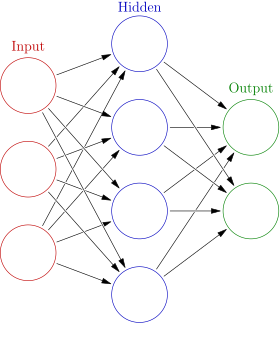
\includegraphics[width=0.5\linewidth]{images/neural_network.png}
    \caption{Neural network visualization}
    \label{fig:neural_network}
\end{figure}

Formally, neural networks are defined as functions of the features $X$ in the form given by the Equation \ref{eq:nn}, where $a_k$ represents the activation function for the k-th layer and the $W_k$ represents the weights for the k-th layer.

\begin{equation}
    h(X) = a_k(a_{k-1}(...a_2(a_1(X \cdot W_1)W_2)...W_{k-1})W_{k})
    \label{eq:nn}
\end{equation}

The activation functions $a_k$ introduce the non-linearity to the model.
One of the most commonly used activation functions are:
\begin{itemize}
    \item $ReLU(x) = max(0, x)$ 
    \item $Softmax(x)_i = \frac{e^{x_i}}{\sum_{j=1}^{J} e^{x_j}}$ 
    \item $Identity(x) = x$ 
\end{itemize}

The weights $W_k$ represents the trainable parameters of the model.
Training of the weights is typically done via a mini-batch stochastic gradient descent (SGD) algorithm.
The first step of this algorithm is to select $m$ observations from the dataset.
These observations, together with the current weights $W$, are then used to evaluate the function $h$, which will give us the predicted values for labels $Y$.
The evaluation of the function $h$ is also called the forward pass.

Then, we calculate the in-sample error $E_{in} = l(h(X), Y)$, using the loss function $l$.
There are many options for the choice of loss function $l$, each dependent on the task at hand, but the most commonly used are mean squared error (MSE) for regression tasks and negative log-likelihood (NLL) for classification tasks.

After calculating the in-sample error $E_{in}$, we will adjust the weights of the model in a way, which lowers the $E_{in}$.
For this purpose, we calculate the gradient $\nabla_W E_{in}$ using the backpropagation.
The backpropagation is an algorithm, which can automatically compute the gradient by using the basic chain rule of differentiation.
After computing the gradient, we can update the weights of our model using the expression $W = W - \alpha \nabla_W E_{in}$, where $\alpha$ is the learning rate controlling the size of the step taken during the update.
To optimize the parameters $W$, we repeat this process many times, until we reach convergence.
The summary of the algorithm can be found in the Note \ref{alg:SGD}.

\begin{enumerate}
    \item initialize $W$ (randomly) and $\alpha$ (to constant)
    \item until convergence
    \begin{enumerate}
        \item sample $m$ observations from dataset
        \item calculate in-sample error $E_{in} = l(h(X), Y)$ of the sampled observations
        \item calculate the gradient $\nabla_W E_{in}$ with backpropragation
        \item update weights $W = W - \alpha \cdot \nabla_W E_{in}$
    \end{enumerate}
    \label{alg:SGD}
\end{enumerate}

After the model has been trained, it can be used to predict new values $Y$ from the new values $X$ simply by using these new values of $X$ in a forward pass.

\subsection{Autoencoders}
Autoencoders are a special type of neural networks that are used to learn a reduced representation of the original data \cite{lauzon2012introduction}.
This is achieved by using a bottleneck, which forces the neural network to compress usually high-dimensional features $X$ to their low-dimensional representation $Z$.

Since we are not given the labels $Y$, we need to redefine our objective slightly.
We define two basic components of the autoencoder, the encoder (ENC) and the decoder (DEC), where both of these components are neural networks.

The encoder's main task is to take the original features $X$ with the dimensionality $d$ and transform it to a new representation $Z$ with dimensionality $p$, where the dimensionality $p$ is usually much smaller than the dimensionality $d$.

The decoder's task is then to take the new representation $Z$ and reconstruct the original features $X$ as well as possible.

This definition of the problem gives us a new objective to minimize, sometimes also called the reconstruction loss, as shown in the Equation \ref{eq:autoencoder}.

\begin{equation}
    E_{in}(X) = l(DEC(ENC(X)), X)
    \label{eq:autoencoder}
\end{equation}

The optimization of this objective can be done, similarly as in the previous case, by using the mini-batch SGD algorithm.
The low-dimensional representation of the data can be obtained after the training simply by using the encoder function (ENC) on the features $X$.

\newpage
\section{Bayesian statistics}
\label{sec:bayes}
% observed data x
Suppose that we are given an observed data $x$.
In Bayesian statistics, we would like to model the observed data by using a Bayesian model.

% Bayesian model
Bayesian models are mathematical models representing our assumptions about the generative process, which created our observed data \cite{mcelreath2018statistical}.
These models can inform us about the important characteristics of our data, such as the likelihood of observing the data, but also the uncertainty that we will observe them.
% probability to represent uncertainty in all parts of a statistical model
% inherent uncertainty that needs to be quantified

% model parameters
Bayesian models usually have some parameters that can be modified and the distribution of the observed data is dependent on these parameters.

For example, a coin toss can be modelled as taking samples from a Bernoulli distribution.
The Bernoulli distribution can produce two possible outcomes and is parametrized by a single parameter, which is equal to the probability of the first outcome. 
% In most cases models only approximate the true process, and may not take into account certain factors influencing the data.

% latent variables z
In Bayesian models, probabilities can be assigned to model parameters.
These probabilistic parameters are then sometimes called latent variables $z$.

Since Bayesian models are generative models, it is possible to generate samples.
% given model and its parameters we can generate the data or figure out what is the probability to see this data
To draw samples, we first need to draw the latent variables $z$ from a prior density $p(z)$.
% but we are in a different position - we know what are the data, but not the parameters
Then we can relate them to the observed data $x$ using the likelihood $p(x|z)$.

% prior probability
The prior density $p(z)$ reflects our belief on the value of the latent variable $z$ before seeing any data.
This can usually be defined via expert knowledge about the process generating the data or we can use priors with maximum entropy \cite{mcelreath2018statistical}. 
After defining priors, we look at the data and update our beliefs about the latent variables so they better reflect the observed data $x$.
% posterior probability
The updated densities are also called posterior densities and the process of updating them is called Bayesian inference.
% Bayesian inference
The Bayesian inference is a flexible extension of maximum likelihood estimation and potentially the most information-efficient method to fit a statistical model.
On the other side, it is also one of the most computationally expensive methods.

The goal of the Bayesian inference is to compute the posterior density of the latent variables $z$ conditioning on the observed data $x$.
The density $p(z|x)$ can be computed using the Bayesian theorem, which can be derived from the joint density of latent variables $z$ and observed data $x$ as shown in the Equation \ref{eq:bias}.

\begin{equation}
    p(z, x) = p(x|z)p(z) = p(z|x)p(x) \implies p(z|x) = \frac{p(x|z) p(z)}{p(x)}
    \label{eq:bias}
\end{equation}

In general, the Bayes theorem formalizes how to compute and update our beliefs in the light of new data.
However, in the complex models, the denominator of the Bayesian theorem is often intractable and therefore we can not do the Bayesian inference directly, but we are forced to approximate it with methods such as Approximate Bayesian computation, Markov chain Monte Carlo or Variational inference.

\subsection{Approximate Bayesian computation (ABC)}
Approximate Bayesian Computation is a mathematically well-founded and conceptually easy method \cite{marin2012approximate}.
Unfortunately, this method is usually very slow in practice and faster methods were developed.
These methods, including the Markov chain Monte Carlo and Variational inference, are trying to achieve the same results using clever tricks.
Sadly, these tricks make understanding and analysis of these methods difficult.
Therefore, we decided to include the Approximate Bayes Computation in this report to illustrate how we can get the posterior density $p(z|x)$ using the prior density $p(z)$ and the data $x$.

\begin{example}
Let us suppose that we have an unfair coin with an unknown probability of landing on the "head" side $\theta$.
We flip this coin 16 times and count how many times it landed on the "head" side.
It lands on the "head" side 6 times, therefore we have $x = 6$.
To model this process, we decide to use the Binomial distribution with parameters 16 and $\theta$ in our generative model.
Also, we do not know which probability $\theta$ is more likely, therefore we assume that the $\theta$ is distributed uniformly at the interval $[0, 1]$.
This will be our prior probability density of $z$.

Our generative model now looks like:
\begin{itemize}
    \item $\theta \sim Unif(0, 1)$
    \item $x \sim Bin(16, \theta)$
\end{itemize}

This model allows us to run the ABC rejection algorithm to approximate the true $\theta$ parameter.
The ABC rejection algorithm consists of these steps:
\begin{enumerate}
    \item Pick a value of $\theta$ at random from ist prior distribution.
    \item Simulate $x$ using the selected value of $\theta$ and $Bin(16, \theta)$.
    \item Reject the simulated data if it is inconsistent with the observed data.
    \item Repeat the step 1.-3. many times.
    \item The posterior density of $\theta$ is now the density created from all non-rejected values of $\theta$.
\end{enumerate}

We show the prior and posterior density of $\theta$ in the Figure \ref{fig:prior_posterior}.
\begin{figure}[H]
    \centering
    \includesvg[width=\linewidth]{images/prior.svg}
    \includesvg[width=\linewidth]{images/posterior.svg}
    \caption{Prior (top) and posterior (bottom) densities of the parameter $\theta$ obtained from the rejection algorithm.}
    \label{fig:prior_posterior}
\end{figure}
\end{example}

\subsection{Markov chain Monte Carlo (MCMC)}
Markov chain Monte Carlo is a family of methods, that has been the dominant paradigm for the approximate Bayesian inference for decades \cite{blei2017statreview}.
In these methods, the first step is to construct an ergodic Markov chain on $z$, with the stationary distribution being equal to the posterior $p(z|x)$.
Then, we perform a random walk on this Markov chain and record the visited states of the Markov chain. 
These states are then used to approximate the posterior density $p(z|x)$.

Usually, it is not hard to construct the desired Markov chain, but it is challenging to determine the number of steps needed to converge to the stationary distribution within an acceptable error \cite{gelman1992inference}.
This problem can be assessed by generating multiple independent chains and checking that the ratio between the inter-chain and intra-chain variances of the parameters is close to 1.

The MCMC methods often tend to move in small steps across the space of all possible values for parameters, which makes them computationally expensive and creates a strong need for a faster approximation of the parameters generating recent big datasets.

\subsection{Variational inference (VI)}
In contrast with the previous methods which use sampling to approximate the posterior density $p(z|x)$, variational inference turns this problem into an optimization problem.

First, we define a family of densities $\mathscr{Q}$ over latent variables $z$ \cite{blei2017statreview}.
As an example, this can be a family of all normal distributions.
Then, we try to find a member $q(z)$ of the family $\mathscr{Q}$ which is closest to the true posterior density $p(z|x)$.
We define the closeness in terms of Kullback–Leibler (KL) divergence, thus the inference can now be formulated as an optimization problem given by the Equation \ref{eq:opt}. 

\begin{equation}
    q^{\ast}(z) = \argmin_{q(z) \in \mathscr{Q}} \KL(q(z) \| p(z|x))
    \label{eq:opt}
\end{equation}

The optimized density $q^{\ast}(z)$ is the best approximation of the posterior density $p(z|x)$.
This optimization process is visualized in the Figure \ref{fig:opt}.

\begin{figure}[H]
    \centering
    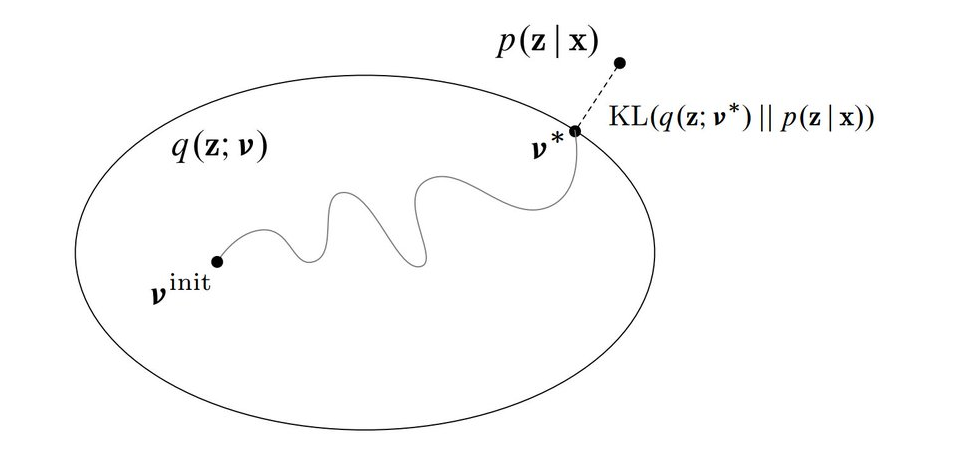
\includegraphics[width=\linewidth]{images/VI.png}
    \caption{Optimization of the KL divergence.}
    \label{fig:opt}
\end{figure}

Unfortunately, the optimization problem \ref{eq:opt} is not solvable, because the KL divergence requires to compute the density p(x).
The density p(x), also called the evidence, is defined in the Equation \ref{eq:pofx} and it is the main reason, why we are doing the approximation of the Bayesian inference and not the Bayesian inference in the first place.

\begin{equation}
    p(x) = \int p(x, z) dz
    \label{eq:pofx}
\end{equation}

To see why KL divergence requires to compute the evidence, we can expand it as shown in the Equation \ref{eq:kl_exp}.

\begin{equation}
    \KL(q(z) \| p(z|x)) = \mathds{E}_{z}[\log q(z)] - \mathds{E}_{z}[\log p(z,x)] + \log p(x).
    \label{eq:kl_exp}
\end{equation}

Because it is not possible to optimize the KL divergence, we will optimize different quantity called the evidence lower bound (ELBO).
The ELBO is defined as the negative KL divergence from $q(z)$ to $p(z|x)$ plus the $\log p(x)$.
This definition ensures that maximizing the ELBO is the same objective as minimizing the KL divergence because the only difference between these two quantities is the reversed sign and added constant.

The ELBO can also be rewritten as a sum of the negative KL divergence from the variational density $q(z)$ to the prior density $p(z)$ and the expected log-likelihood of the data $x$ conditioned on the latent variables $z$.
This formulation of the problem reveals a different interpretation of the ELBO measure.
The first term promotes the posterior densities $q(z)$ which are close to the prior densities $q(z)$.
The second term promotes the posterior densities $q(z)$ which explain the observed data $x$ well.
The formal notation of the ELBO formulations can be found in the Equation \ref{eq:elbo}.

\begin{equation}
\begin{split}
    \ELBO(q) &= - \mathds{E}_{z}[\log q(z)] + \mathds{E}_{z}[\log p(z,x)] - \log p(x) + \log p(x) \\
             &= - \mathds{E}_{z}[\log q(z)] + \mathds{E}_{z}[\log p(z,x)] \\
             &= - \mathds{E}_{z}[\log q(z)] + \mathds{E}_{z}[\log p(z)] + \mathds{E}_{z}[\log p(x|z)]   \\
             &= - \KL(q(z) \| p(z)) + \mathds{E}_{z}[\log p(x|z)] \\
\end{split}
\label{eq:elbo}
\end{equation}

Another useful property of the ELBO is that it bounds the log evidence $p(x)$ from the bottom, hence the name evidence lower bound.
It is shown, using the fact that the KL divergence is larger or equal to zero, in the Equation \ref{eq:logpx}.

\begin{equation}
\begin{split}
    \log p(x) &= \KL(q(z) \| p(z|x)) + \ELBO(q) \\
              &\geq \ELBO(q)
\end{split}
\label{eq:logpx}
\end{equation}

All of these properties make ELBO a good candidate for optimization.
The optimization is usually much faster than the previous methods, which makes it a suitable method for big datasets.
Unfortunately, the ELBO is not a convex function.
Therefore, we do not have any theoretical guarantees to arrive at a global optimum.
Nevertheless, the results are usually good enough in practice and they are often better than what we would be able to obtain from other approximation methods on big datasets.

% $\ELBO$ is not convex. % https://www.youtube.com/watch?v=ogdv_6dbvVQ
% a stochastic approximation method - robbins and monroe - 1951
% guarantees to converge to local optimum - bottou, 1996

% Using a Bernoulli VAE on Real-Valued Observations
% http://ruishu.io/2018/03/19/bernoulli-vae/

% How to Train Deep Variational Autoencoders and Probabilistic Ladder Networks
% https://orbit.dtu.dk/files/121765928/1602.02282.pdf

\newpage
\section{Variational Autoencoder (VAE)}
As the name suggests, the Variational Autoencoder (VAE) is a combination of the autoencoder described in the section \ref{sec:nn} and the variational inference in the section \ref{sec:bayes} \cite{kingma2013}.

The main goal here is to find the posterior density $p(z|x)$ for each sample $x$ from the dataset $X$.
We are assuming that the dataset $X$ consists of $N$ independent and identically distributed (i.i.d.) samples of continuous variable $x$ and is too large to be used in optimization with methods such as Monte Carlo Expectation-Maximization algorithm.
Furthermore, we assume that sample $x$ is generated from conditional density $p_{\theta}(x|z)$ and that the latent variable $z$ is drawn from prior density $p_{\theta}(z)$.
Moreover, the densities $p_{\theta}(x|z)$ and $p_{\theta}(z)$ are from parametric families and their probability density functions are differentiable almost everywhere.
Finally, the marginal likelihood $p_{\theta}(x)$ is intractable and the parameters $\theta$ and the latent variable $z$ are unknown.

To solve this problem, we define two components, the probabilistic encoder $q_{\phi}(z|x)$ and the probabilistic decoder $p_{\theta}(x|z)$, similarly how we did in a standard autoencoder.
The difference between the standard encoder and the probabilistic encoder is that the probabilistic encoder's output is a probability distribution over $z$.
Likewise, the probabilistic decoder's output is a distribution over $x$.

The forward pass over this model would then consist of feeding the sample $x$ to the probabilistic encoder $q_{\phi}(z|x)$ and producing the distribution over $z$.
Next, we would draw a sample from this distribution, which would give us the latent variable $z$.
The latent variable $z$ would be then used as an input to the probabilistic decoder $p_{\theta}(x|z)$, which would produce a distribution over $x$.

Unfortunately, drawing a latent variable $z$ from its distribution is a stochastic process, thus it is not differentiable and would not allow us to perform a backward pass in the same way as in standard autoencoders.
To solve this issue, we introduce a reparametrization trick.
In the reparametrization trick, we express a latent variable $z$ as a deterministic variable $z = g_{\phi}(\epsilon, x)$, where the $\epsilon$ is known as an auxiliary variable with independent marginal density and the function $g$ characterizes the differentiable transformation needed to transform $\epsilon$ to $z$. 

The reparametrization trick limits the families which can be used to approximate the prior density $p(z)$ to three main classes:
\begin{itemize}
    \item Family of distributions with tractable inverse cumulative distribution function (CDF). In this case, we let $\epsilon \sim Unif[0, 1]$ and $g_{\phi}(\epsilon, x)$ to be the inverse CDF of $q_{\phi}(z|x)$.
    \item The "location-scale" family of distributions. In this case, we let $\epsilon$ to be drawn from the standardized distribution of this family and $g_{\phi}(\epsilon, x)$ to be equal to $location + scale \cdot \epsilon$.
    \item The family of distribution, which are composed of the previous two cases. In this case, the transformation is the composition of the corresponding transformations as well.
    \label{list:families}
\end{itemize}

\newpage
Since we would like to optimize this reparametrized model with standard SGD technique, we also need to define the loss function.
Here, we make use of the $ELBO$ measure defined in the section \ref{sec:bayes}.
Rewriting the second line of the Equation \ref{eq:elbo} to our encoder-decoder notation yields the Equation \ref{eq:elbo_vae}.

\begin{equation}
    \mathcal{L}(\theta, \phi; x_i) = \mathds{E}_{q_{\phi}(z|x)}(\log p_{\theta}(x, z) - \log q_{\phi}(z|x))
    \label{eq:elbo_vae}
\end{equation}

Thanks to the reparametrization trick we can estimate the ELBO quantity with a new quantity, Stochastic Gradient Variational Bayes (SGVB), as shown in the Equation \ref{eq:SGVB_a}. 
\begin{equation}
    \widetilde{\mathcal{L}}^A(\theta, \phi; x_i) = \frac{1}{L}\sum_{l=1}^{L} \log p_{\theta}(x_i, g_{\phi}(\epsilon_{il}, x_i)) - \log q_{\phi}(g_{\phi}(\epsilon_{il}, x_i)|x_i))
    \label{eq:SGVB_a}
\end{equation}

This estimate can be used for all families of distributions defined in the List \ref{list:families}, but often the KL divergence term from the fourth line of the Equation \ref{eq:elbo} can be computed analytically.
This would yield a new SGVB estimate as shown in the Equation \ref{eq:SGVB_b}.

\begin{equation}
\begin{split}
    \widetilde{\mathcal{L}}^B(\theta, \phi; x_i) &= -\KL(q_{\phi}(z|x_i) \| p_{\theta}(z)) + \frac{1}{L}\sum_{l=1}^{L} \log p_{\theta}(x_i|g_{\phi}(\epsilon_{il}, x_i)) \\
\end{split}
\label{eq:SGVB_b}
\end{equation}

Moreover, this second estimate typically has lower variance than the former one.
Since the basic stochastic gradient descent algorithm produces noisy updates for the weights, we would like to use mini-batch SGD.
For this purpose, we need to define an estimate based on the mini-batches with $M$ data points as shown in the Equation \ref{eq:SGVB_mb}.

\begin{equation}
    \widetilde{\mathcal{L}}^M(\theta, \phi; X^M) = \frac{N}{M} \sum_{i=1}^{M} \widetilde{\mathcal{L}}(\theta, \phi; x_i)
    \label{eq:SGVB_mb}
\end{equation}

The training of the variational autoencoder can now be achieved simply by maximizing these SGVB measures using standard techniques such as SGD.